\documentclass[11pt,a4paper]{article}

\usepackage{Act}
\usepackage{listings}

\begin{document}
\input{\detokenize{/home/fenarius/Travail/Cours/Commun/latex/Macros.tex}}

\DevoirNSI{Révisions}{\Term}\vspace{0.2cm}
\pythonmode


\Exo{Quelques commandes}{}\\
Compléter le tableau suivant qui donne quelques commandes et leur signification
\begin{center}
    \renewcommand{\arraystretch}{1.5}
\begin{tabularx}{0.95\textwidth}{|c|X|}
    \hline
    {\tt cd /home/toto} & Se déplacer dans le répertoire {\tt /home/toto} \\
    \hline
    {\tt .............} & Créer le répertoire {\tt exo1} \\
    \hline
    {\tt .............} & Créer le fichier vide  {\tt rep.txt} \\
    \hline
    {\tt chmod g-w rep.txt} & ................................. \\
    \hline
    {\tt .................} & Ajouter le droit d'exécution pour l'utilisateur sur le fichier {\tt rep.txt} \\
    \hline
    {\tt .................} & Renommer le fichier {\tt rep.txt} en {\tt reponses.txt} \\
    \hline
    {\tt cp reponses.txt \~{}/Sauvegardes} & ......................................... \\
    \hline
    {\tt .................} & Supprimer le fichier {\tt reponses.txt} \\
    \hline
\end{tabularx}
\end{center}

\vspace{0.5cm}

\Exo{Programme turtle} \\
On donne ci-dessous le squelette d'un programme Python utilisant le module turtle
\begin{lstlisting}
import turtle

# Création du "papier" et du "crayon"
crayon = turtle.Turtle()
papier = turtle.Screen()
papier.setup(width=500,height=500)

# Attends un clic pour fermer la fenêtre de dessin
papier.exitonclick()
\end{lstlisting}
\QListe
\item Ecrire une fonction {\tt rectangle} telle que {\tt rectangle(x,y,largeur,longueur)}  construit avec la tortue {\tt crayon} un rectangle de dimensions {\tt largeur}$\times${\tt longueur} dont le coin inférieur droit se trouve au point de coordonnées {\tt (x,y)}
\item En utilisant la fonction ci-dessus ainsi qu'une boucle et une instruction conditionnelle, réaliser le dessin suivant :
\begin{center}
    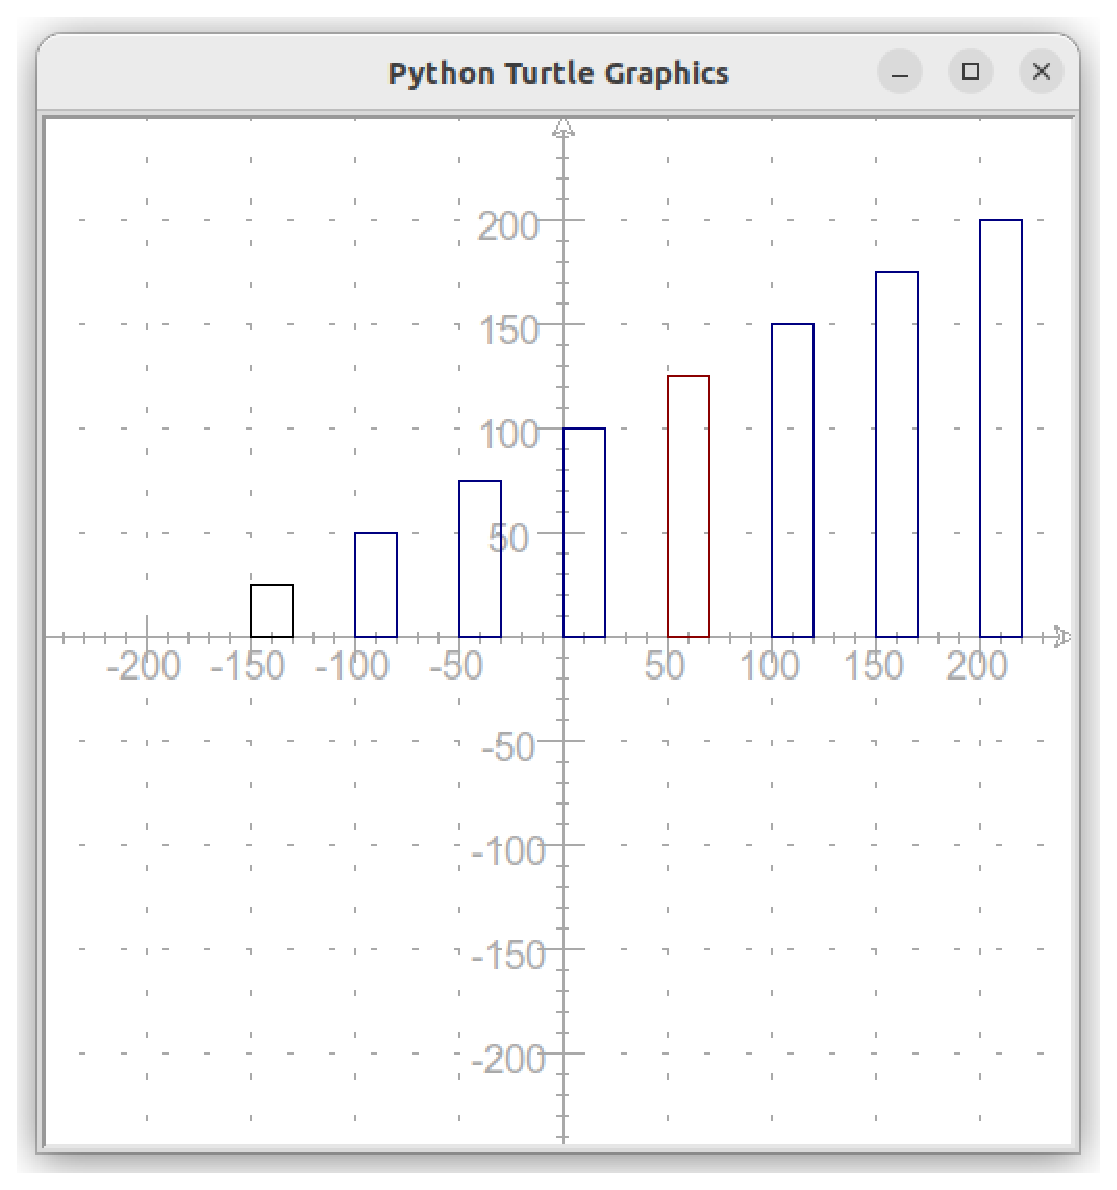
\includegraphics[width=200px]{TermD1-1.eps}
\end{center}
\FinListe

\Exo{Création de liste}{}\\
Ecrire un programme python permettant de créer :
\QListe
\item par répétition, la liste {\tt liste1} qui contient 15 fois le l'entier 28.
\item par ajout successif, la liste {\tt liste2} qui contient les entiers de 1 à 100.
\item par compréhension, la liste {\tt liste3} qui contient les 20 premières puissances positives de 2, c'est à dire $2^0, 2^1, \dots 2^{19}$.
\FinListe
\end{document}

